\documentclass[aspectratio=169]{beamer}  % avec animation
%\documentclass[aspectratio=169,handout]{beamer}  % sans animation
\usepackage[T1]{fontenc}
\usepackage[utf8]{inputenc}
\usepackage{lmodern}
\usepackage[french]{babel}
%\usepackage{appendixnumberbeamer}

%\usetheme{Madrid}
%\usetheme{Berlin}
%\usetheme{Antibes}
%\usetheme{Ilmenau}
\usetheme{Luebeck}
%%%\usetheme{AnnArbor}
%\usetheme{Dresden}
%\useinnertheme{rectangles}
\useinnertheme{rounded}
\useoutertheme{infolines}

\beamertemplatenavigationsymbolsempty

\title{Attaque des contrôles d'accès}
\subtitle{Présentation de STI}
\author[Wojciechowski, Dössegger et Roch]{Cassandre Wojciechowski \and Gwendoline Dössegger \and Gabriel Roch}
\date{20 novembre 2020}
\institute[HEIG]{Haute École d'Ingénierie et de Gestion du Canton de Vaud}

 \AtBeginSection[]
 {
   \begin{frame}[noframenumbering]
     \sectionpage
   \end{frame}
   \begin{frame}[noframenumbering]
     \frametitle{Sommaire}
     \tableofcontents[currentsection,sectionstyle=show/shaded,subsectionstyle=show/show/hide]
   \end{frame}
 }
% \AtBeginSubsection[]
% {
%   \begin{frame}
%     \frametitle{Table of Contents}
%     \tableofcontents[currentsection,currentsubsection]
%   \end{frame}
% }

\newcommand{\demo}{
\begin{frame}[noframenumbering]
  \begin{center}
    \Huge Demo
  \end{center}
\end{frame}}

\begin{document}

\begin{frame}[plain,noframenumbering]
  \titlepage
\end{frame}

\begin{frame}[noframenumbering]
  \frametitle{Sommaire}
  \begin{columns}[c]
    \column{.45\textwidth}
      \tableofcontents[subsectionstyle=hide]
    \column{.45\textwidth}
      \begin{block}{Exemple ou note}
        \vspace{1em}
      \end{block}
      \begin{alertblock}{Attaque}
        \vspace{1em}
      \end{alertblock}
      \begin{exampleblock}{Sécurisation}
        \vspace{1em}
      \end{exampleblock}
  \end{columns}
\end{frame}

\begin{frame}
  \frametitle{Qu'est-ce que les contrôles d'accès (access controls) ?}
  \begin{itemize}
    \item Vérification du niveau d'accréditation (vertical)
    \item Vérification de l'identité de l'utilisateur (horizontal)
    \item Restriction de l'accès en fonction des vérifications ci-dessus
  \end{itemize}
%   Les contrôles d'accès sont des vérifications effectuées afin de restreindre les accès aux ressources selon les niveaux d'accréditation (vertical) et selon l'identité (horizontal) de l'utilisateur. 
\end{frame}

\section{Vulnérabilités communes}
\subsection*{Introduction}

\begin{frame}
  \frametitle{Vulnérabilités communes}
  \begin{itemize}
    \item Vulnérabilités verticales
    \item Vulnérabilités horizontales
    \item Vulnérabilités dépendant du contexte
  \end{itemize}
\end{frame}
\begin{frame}
  \frametitle{Vulnérabilités verticales}
  \begin{columns}[c]
    \column{.45\textwidth}
      \begin{description}
        \item[Vulnérabilité] \hfill \\ Utiliser des fonctions de l'application quand notre rôle ne le permet normalement pas.
        \item[Type d'attaque] \hfill \\ Escalade de privilèges verticale --- \emph{vertical privilege esalation}
      \end{description}
      \begin{block}{Exemple d'attaque}
        Devenir administrateur quand on est un utilisateur lambda.
      \end{block}
    \column{.45\textwidth}
      \begin{center}
        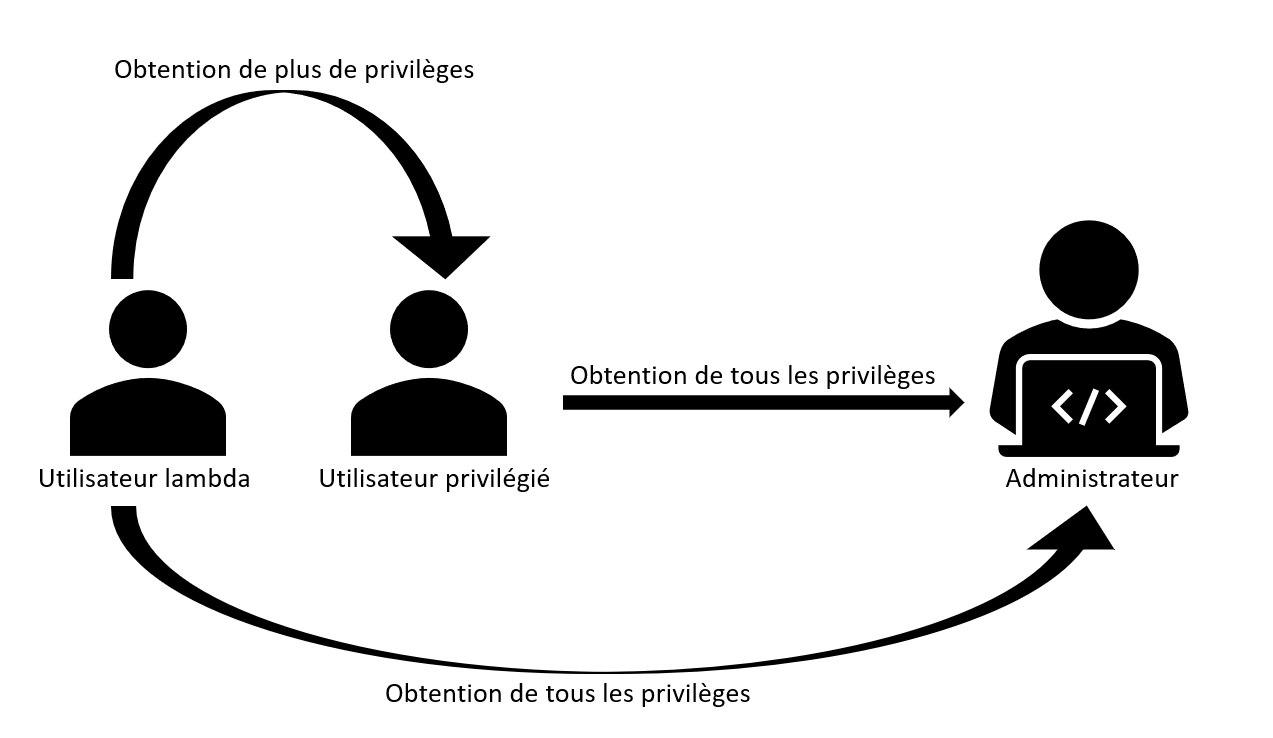
\includegraphics[width=\textwidth]{escalade-vert}
      \end{center}
  \end{columns}
\end{frame}
\begin{frame}
  \frametitle{Vulnérabilités horizontales}
  \begin{columns}[c]
    \column{.45\textwidth}
      \begin{description}
        \item[Vulnérabilité] \hfill \\ Accéder aux ressources d'autres utilisateurs du même niveau.
        \item[Type d'attaque] \hfill \\ Escalade de privilèges horizontale --- \emph{horizontal privilege esalation}
      \end{description}
      \begin{block}{Exemple d'attaque}
        Un utilisateur lambda peut lire les emails d'un autre utilisateur lambda
      \end{block}
    \column{.45\textwidth}
      \begin{center}
        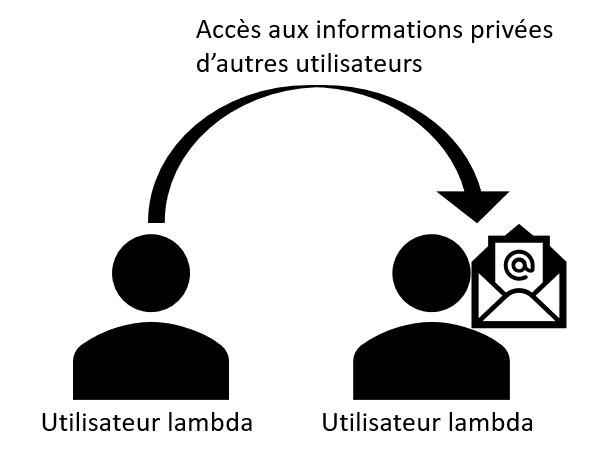
\includegraphics[width=\textwidth]{escalade-hor}
      \end{center} 
  \end{columns}
\end{frame}
\begin{frame}
  \frametitle{Vulnérabilités dépendant du contexte}
  \begin{columns}[c]
    \column{.45\textwidth}
      \begin{description}
        \item[Vulnérabilité] \hfill \\ Le contrôle d'accès ne prend pas en compte l'état actuel de l'application
        %L'accès des utilisateurs est limité à ce qui est autorisé selon l'état actuel de l'application
        \item[Type d'attaque] \hfill \\ Accès hors du flux d'exécution normal --- \emph{business logic exploitation}
      \end{description}
    \column{.45\textwidth}
      \begin{block}{Exemple d'attaque}
        Accéder à une page de paiement en ligne sans passer par l'étape de calcul des frais de port.\\
        Sauter des étapes de vérification normalement obligatoires.
      \end{block}
  \end{columns}
  \begin{center}
    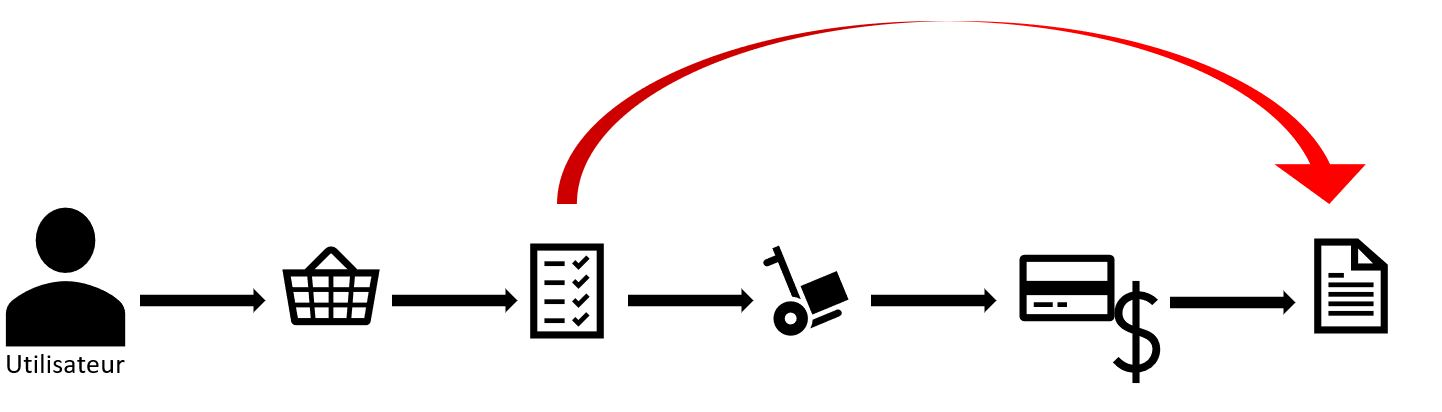
\includegraphics[width=22em]{escalade-hors-flux}
  \end{center}
\end{frame}



\subsection{Fonctionnalités non-protégées}

\begin{frame}
  \frametitle{Contrôles d'accès par connaissance d'URL}
  \begin{columns}[c]
    \column{.45\textwidth}
      \begin{itemize}[<1->]
        \item Certains sites masquent l'URL de la page d'admin pour les utilisateurs
        \item Le contrôle d'accès n'est pas toujours fait sur les pages d'admin
      \end{itemize}
      \begin{exampleblock}{Sécurisation}<3->
        \begin{itemize}
          \item Ne pas se baser sur l'ignorance des utilisateurs pour les URLs et les identifiants des documents
        \end{itemize}
      \end{exampleblock}
    \column{.45\textwidth}
      \begin{block}{L'URL n'est pas secret}<2->
        Le fait que l'URL ne soit pas affichée n'empêche pas l'attaquant d'y accéder, il va pouvoir la trouver autre part (essayer des URLs habituelles, outils de bruteforce, dans le code source, sur internet, ...)
        
        D'autres moyens peuvent également être utilisés car une URL n'est jamais traitée comme confidentielle par les logiciels et serveurs.
      \end{block}
  \end{columns}
\end{frame}

\begin{frame}
  \frametitle{Découvrir une URL d'administration}
  \begin{alertblock}{Attaque}
    \begin{itemize}
      \item Commentaires dans le code source,
      \item Affichage à l'écran, 
      \item Historique des navigateurs, favoris,
      \item Envoi du lien par e-mail (ou autres outils) par certains utilisateurs,
      \item Logs (clients, serveurs, proxys), 
      \item Scripts de génération des menus.
    \end{itemize}
  \end{alertblock}
\end{frame}

\demo
  
\subsection{API}
\begin{frame}
  \frametitle{Accès direct à l'API}
  Sur certains sites, les API ne font pas les mêmes contrôles d'accès que pour les pages "standards"
  \begin{columns}[T]
    \column{.45\textwidth}
      \begin{alertblock}{Attaque}
        \begin{itemize}
          \item Analyse des requêtes faites par le navigateur
          \item Test des URLs standards
          \item Test les ressources devinables
        \end{itemize}
      \end{alertblock}
    \column{.45\textwidth}
      \begin{exampleblock}{Sécurisation}
        \begin{itemize}
          \item L'API doit être sécurisée de la même manière que les pages standards de modification, car les mêmes risques s'appliquent
          \item Les fonctions privilégiées doivent vérifier les privilèges de l’utilisateur.
        \end{itemize}
      \end{exampleblock}
  \end{columns}
\end{frame}

\subsection{Contrôle basées sur les identifiants}
\begin{frame}
  \frametitle{Contrôle basées sur les identifiants}
  Certains sites permettent l'accès à des fonctionnalités en fonction de l'ID d'une ressource (statique ou dynamique).
  \vspace{2em}
  \begin{itemize}
    \item Les IDs peuvent être devinés.
    \item Les GUID n'améliorent que peu la sécurité (prévisibles).
    \item Les ID peuvent être affichés ailleurs.
  \end{itemize}
\end{frame}
\begin{frame}
  \frametitle{Contrôles basés sur les identifiants}
  \begin{columns}[T]
    \column{.45\textwidth}
      \begin{alertblock}{Attaque}
        \begin{itemize}
          \item Deviner les identifiants
          \item Les identifiants sont les mêmes quelle que soit l’action
          \item Accès à une ressource connue avec un compte moins privilégié (et même sans s'identifier)
        \end{itemize}
      \end{alertblock}
    \column{.45\textwidth}
      \begin{exampleblock}{Sécurisation}
        \begin{itemize}
          \item Vérifier les droits d'accès à la ressource de l'utilisateur.
          \item Vérifier que l'utilisateur a le droit de faire l'action demandée
        \end{itemize}
      \end{exampleblock}
  \end{columns}
\end{frame}
\subsection{Contrôle basé sur la requête}
\begin{frame}
  \frametitle{Contrôle basé sur la requête}
  \begin{columns}[c]
    \column{.45\textwidth}
      \begin{itemize}
        \item Les contrôles d'accès peuvent ne pas être effectués par l'application mais par l'infrastructure (par ex. Apache)
        \item Apache peut valider une requête avec les critères suivants
        \begin{itemize}
          \item L'URL demandée (\texttt{/admin}, \texttt{/image})
          \item Le type de fichier demandé
          \item La méthode HTTP utilisée (\texttt{GET}, \texttt{POST}, \texttt{HEAD}, ...)
          \item Les identifiants de l'utilisateur
          \item Les cookies (admin=true)
        \end{itemize}
      \end{itemize}
    \column{.45\textwidth}
      \begin{block}{Methode HTTP particulière}
        Une requête \texttt{HEAD} doit renvoyer les mêmes en-têtes que \texttt{GET}, mais sans le corps du message. Pour cela, les mêmes scripts que pour GET sont généralement executés.
      \end{block}
      \begin{block}{Methode HTTP non-standard}
        Les requêtes HTTP non-standards (\texttt{DELETE}, \texttt{TOTO}, ...) peuvent également être traitées par les mêmes scripts.
      \end{block}
  \end{columns}
\end{frame}
\begin{frame}
  \frametitle{Contrôle basé sur la requête}
  \begin{columns}[T]
    \column{.45\textwidth}
      \begin{alertblock}{Attaque}
        \begin{itemize}
          \item Est-ce qu'une requête HEAD fonctionne?
          \item Est-ce qu'une méthode HTTP non-valide fonctionne?
          \item Est-ce que les privilèges sont les mêmes que pour l'application?
          \item Ce type de contrôle peut également être mis en place pour les pages dynamiques du site.
        \end{itemize}
      \end{alertblock}
    \column{.45\textwidth}
      \begin{exampleblock}{Sécurisation}
        \begin{itemize}
          \item Faire attention lors de la configuration
          \item Passer par un script qui renvoie le fichier après authentification (le fichier original étant innacessible en HTTP)
        \end{itemize}
      \end{exampleblock}
  \end{columns}
\end{frame}

\demo

\subsection{Fonctions en plusieurs étapes}
\begin{frame}
  \frametitle{Fonctions en plusieurs étapes}
  \begin{block}{Exemple de réception de matériel}
    \begin{enumerate}
        \item enregistrement de la facture,
        \item sélection des comptes débiteurs,
        \item mise à jour du stock,
        \item validation du paiement.
    \end{enumerate}
  \end{block}
\end{frame}
\begin{frame}
  \frametitle{Fonctions en plusieurs étapes}  
  \begin{itemize}
    \item Contrôles d'accès à chaque étape.
    \item Vérification de toutes les étapes précedentes à chaque fois.
  \end{itemize}
  \begin{columns}[T]
    \column{.45\textwidth}
      \begin{alertblock}{Attaque}
        \begin{itemize}
          \item Validation finale directe
          \item Bypass d'une étape
          \item Modification du header \texttt{REFERER}
        \end{itemize}
      \end{alertblock}
    \column{.45\textwidth}
      \begin{exampleblock}{Sécurisation}
        \begin{itemize}
          \item Ne pas faire confiance aux utilisateurs pour utiliser les fonctionnalités comme elles ont été prévues
          \item Tout revérifier à chaque étape
          \item Le header \texttt{REFERER} doit être considéré comme non-sécurisé
        \end{itemize}
      \end{exampleblock}
  \end{columns}
  
  %En cas de paiement par exemple, il vaut mieux revérifier toutes les informations lors de la dernière étape, il ne suffit pas de transmettre en champs cachés les informations, car elles peuvent être interceptées et modifiées par un attaquant.
\end{frame}

\demo

\subsection{Méthodes de contrôles d'accès non sécurisées}

\begin{frame}
  \frametitle{Contrôles d'accès basés sur des paramètres}
  L'information concernant le rôle ou le niveau d'accès de l'utilisateur est transmis par :
  \begin{itemize}
    \item des cookies
    \item un champ masqué dans le formulaire
    \item un paramètre de la requête
    \item une information dans l'URL
  \end{itemize}
  \vspace*{1em}
  Ces techniques ne sont pas sécurisées car un attaquant peut modifier ces champs et usurper l'identité de l'administrateur.
  \vspace*{1em}
  \begin{exampleblock}{Sécurisation}
    \begin{itemize}
      \item Ne pas faire confiance aux paramètres envoyés par les utilisateurs
    \end{itemize}
  \end{exampleblock}
\end{frame}


\begin{frame}
  \frametitle{Contrôles d'accès basés sur la géolocalisation}
  \begin{columns}[T]
    \column{.45\textwidth}
      Un utilisateur peut modifier sa géolocalisation perçue par le serveur
      \begin{itemize}
        \item VPN
        \item Proxy web
        \item En-tête HTTP X-Forwarded-For
      \end{itemize}
    \column{.45\textwidth}
      \begin{exampleblock}{Sécurisation}
        \begin{itemize}
          \item Ne pas partir du principe que la localisation est juste
        \end{itemize}
      \end{exampleblock}
  \end{columns}
\end{frame}

\subsection{Attaque avec différents comptes}

\begin{frame}
  \frametitle{Comparer différents comptes}
  \begin{alertblock}{Attaque}
    \begin{itemize}
      \item Tester les URLs obtenues à partir d'un compte privilégié avec un compte moins privilégié.
      \item Cartographier le site avec un logiciel comme Burp, pour détecter des URLs non-affichées.
      \item Il faut potentiellement compléter les outils automatiques avec nos connaissances
    \end{itemize}
  \end{alertblock}
\end{frame}


\section{Les bonnes pratiques}
\subsection{En général}
\begin{frame}
  \frametitle{Les bonnes pratiques}
  \begin{exampleblock}{}
    \begin{itemize}
      \item Ne pas laisser des fonctionnalités non utilisées
    \end{itemize}
  \end{exampleblock}
  \pause
  \begin{exampleblock}{}
    \begin{itemize}
      \item Ne pas faire confiance aux utilisateurs pour utiliser les fonctionnalités comme elles ont été prévues
      \item Ne pas faire confiance aux utilisateurs pour ne pas détourner les données transmises par le côté client
      \item Il ne faut faire confiance qu'aux données provenant du côté serveur, et non du côté client. Il faut revalider les identifiants à chaque transmission de données
    \end{itemize}
  \end{exampleblock}
  \pause
  \begin{exampleblock}{}
    \begin{itemize}
      \item Evaluer et documenter les contrôles d'accès pour chaque partie de l'application (pour les fonctionnalités et les ressources)
    \end{itemize}
  \end{exampleblock}
  \pause
  \begin{exampleblock}{}
    \begin{itemize}
      \item Toutes les décisions d'autorisation doivent être prises à partir de la session de l'utilisateur
    \end{itemize}
  \end{exampleblock}
\end{frame}

\begin{frame}
  \frametitle{Les bonnes pratiques}
  \begin{exampleblock}{}
    \begin{itemize}
      \item Utiliser un composant central à l'application pour vérifier tous les contrôles d'accès
      \item Utiliser ce composant central pour valider toutes les requêtes client
      \begin{itemize}
        \item Plus grande clarté des contrôles d'accès
        \item Meilleure maintenabilité (plus efficace et sûr)
        \item Plus adaptable
        \item Moins d'erreurs et d'omissions
      \end{itemize}
    \end{itemize}
  \end{exampleblock}
  \pause
  \begin{exampleblock}{}
    \begin{itemize}
      \item Utiliser des techniques de programmation pour forcer le contrôle d'accès à être effectué et éviter que le développeur passe outre
    \end{itemize}
  \end{exampleblock}
  \pause
  \begin{exampleblock}{}
    \begin{itemize}
      \item Pour les parties sensibles de l'application, effectuer des contrôles supplémentaires, par exemple basés sur l'adresse IP
    \end{itemize}
  \end{exampleblock}
\end{frame}
\begin{frame}
  \frametitle{Les bonnes pratiques}
  \begin{exampleblock}{}
    \begin{itemize}
      \item Accès à des fichiers statiques : 
      \begin{itemize}
        \item - Accès indirect en passant un nom de fichier à une page dynamique côté serveur qui va implémenter un contrôle d'accès et retourner le fichier (pas rediriger dessus, car cela ne mettrait en place aucun contrôle)
        \item - Utiliser l'authentification HTTP et d'autres fonctionnalités du serveur d'application pour contrôler l'authentification (cela risque de faire une vérification différente de celle du composant central, il faut donc s'assurer que cela soit consistant)
      \end{itemize}
    \end{itemize}
  \end{exampleblock}
  \pause
  \begin{alertblock}{}
    \begin{itemize}
      \item Pour des actions critiques, il faut ré-authentifier l'utilisateur à chaque transaction et utiliser un système d'authentification multi-facteurs
    \end{itemize}
  \end{alertblock}
  \pause
  \begin{exampleblock}{}
    \begin{itemize}
      \item Logger toutes les actions effectuées quand des données sensibles sont concernées
    \end{itemize}
  \end{exampleblock}
\end{frame}

\subsection{Application multi-tiers}
\begin{frame}
  \frametitle{Les bonnes pratiques}
  \framesubtitle{Application multi-tiers}
  \begin{exampleblock}{}
    \begin{itemize}
      \item Mise en place de contrôles à chaque couche (si une couche est compromise, les autres ne le sont pas forcement)
      \item Le serveur de l'application peut contrôler les URLs selon le rôle de l'utilisateur
      \item L'application peut utiliser un compte de base de données séparé avec des privilèges limités pour chaque type d'utilisateur (privilèges en lecture-seule) et spécifier précisément quelles tables sont accessibles
      \item Utiliser un compte système avec des privilèges limités pour chaque composant
    \end{itemize}
  \end{exampleblock}
\end{frame}

\begin{frame}
  \frametitle{Modèle de contrôle d'accès}
  \begin{center}
    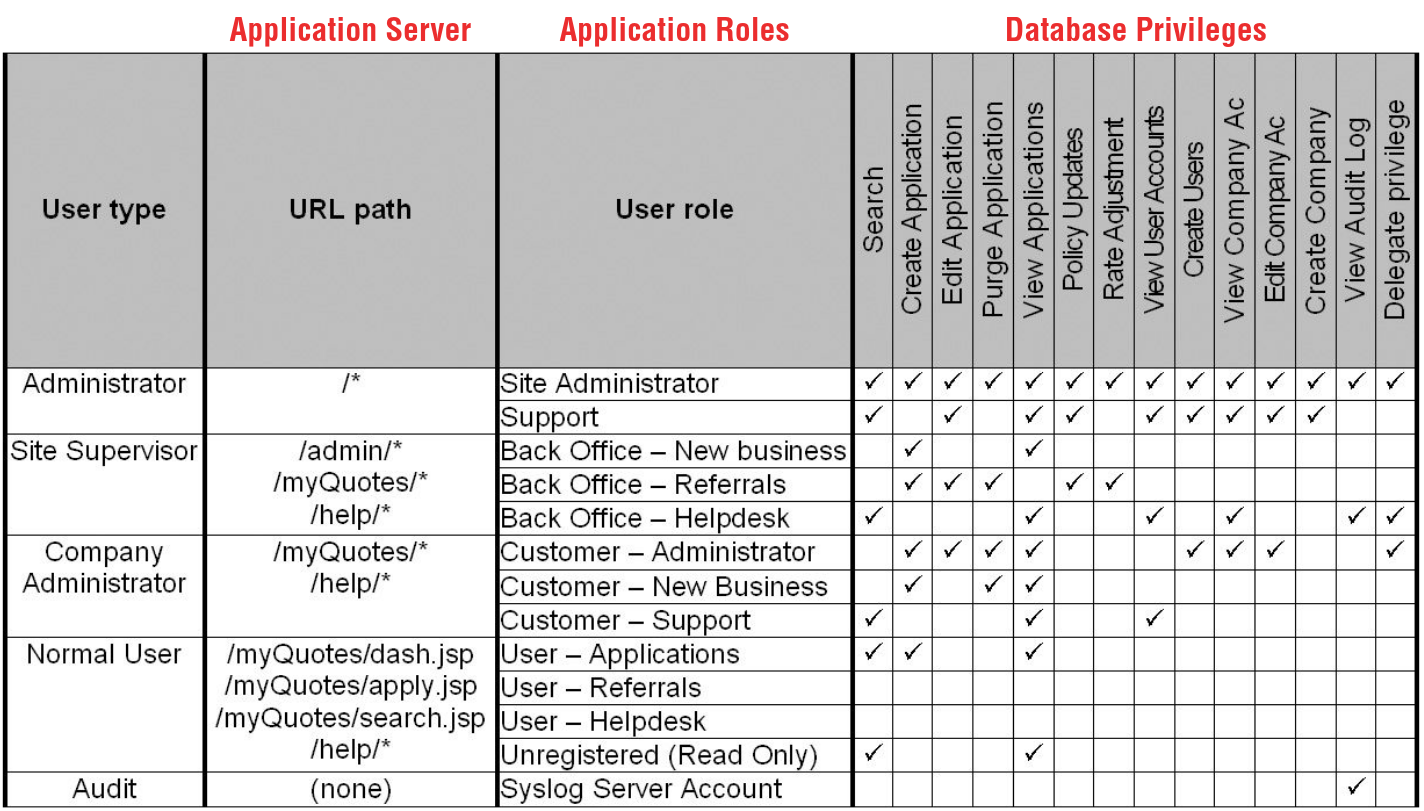
\includegraphics[height=18em]{matrice-droit}
  \end{center}
\end{frame}

\begin{frame}
  \frametitle{Modèle de contrôle d'accès}
  \begin{itemize}
    \item Via des techniques de programmation
    \begin{itemize}
      \item une matrice de droits est stockée dans la base de données 
      \item le programme se charge d'appliquer les contrôles (avec un algorithme aussi complexe que nécessaire)
    \end{itemize}
    \pause
    \item A la discrétion de l'administrateur (discretionary access control DAC)
    \begin{itemize}
      \item l'administrateur peut donner explicitement des privilèges à d'autres utilisateurs pour des ressources auxquelles ils ont accès
      \item modèle fermé : white list
      \item modèle ouvert : black list
    \end{itemize}
    \pause
    \item Basés sur des rôles (role-based access control RBAC)
    \begin{itemize}
      \item chaque rôle donne accès à certains privilèges, pas trop de rôles, ni trop peu, il faut que cela reste gérable et sécurisé
    \end{itemize}
    \pause
    \item Via un composant externe
    \begin{itemize}
      \item utilisation d'un compte de base de données différent pour les groupes d'utilisateurs afin de limiter leurs droits
    \end{itemize}
  \end{itemize}
\end{frame}

\end{document}
